In this section, the Kubernetes mechanisms for resource management are evaluated through a series of experiments. The first experiment aims to demonstrate the effects requests and limits. In the second experiment, a pod is added to the cluster and the effects of different request and limit configurations are evaluated. The impact of bursty workloads is described in the third experiment. The remainder of the experiments describe the effects of adding an HPA to the cluster.


\subsection{Experiment 1: Determining the effects of request and limit configurations}
If there is just one pod scheduled on a node, and if that pod has no limits set, then it should be able to use all of the nodes resources. The goal of this experiment is to validate this hypothesis using a  Cassandra application.

\subsubsection{Setup}
Before performing any experiments, the expected performance of the Cassandra application needs to be defined. This can be described in an SLO as follows:

\begin{slo}
95\% of the requests sent to the Cassandra application must be handled within 150ms, as measured by the experiment controller.
\end{slo}

The Cassandra application is deployed on the second worker node with a CPU and memory request of respectively \textit{1500m} and \textit{2GiB}. No limits are set. In this experiment, the experiment controller sends an increasing amount of requests to the Cassandra application, starting at 100 requests per second up to 600 requests per second, increasing with 50 requests per run. Each run lasts for 600 seconds. Heapster monitors the resource usage and the experiment controller records the latency of each request.

\subsubsection{Results}
Figure \ref{fig:lat-cas-li} shows the 95th percentile latencies of the requests. At around 400 requests per second, they exceed 150ms, violating the SLO. Figure \ref{fig:cpu-cas-li} shows the CPU usage of the Cassandra application and the node on which it is deployed. It illustrates that at around the same amount of requests per second, the node uses all of its available CPU, as 2.0K millicores equals 2 CPUs. This shows that the bottleneck is indeed the CPU. Furthermore, Figure \ref{fig:cpu-cas-li} shows that the Cassandra application is able to use almost all of the overprovisioned resources. This in in line with expectations, as the resources on the node are only contended by the Cassandra application.

\begin{figure}
\centering
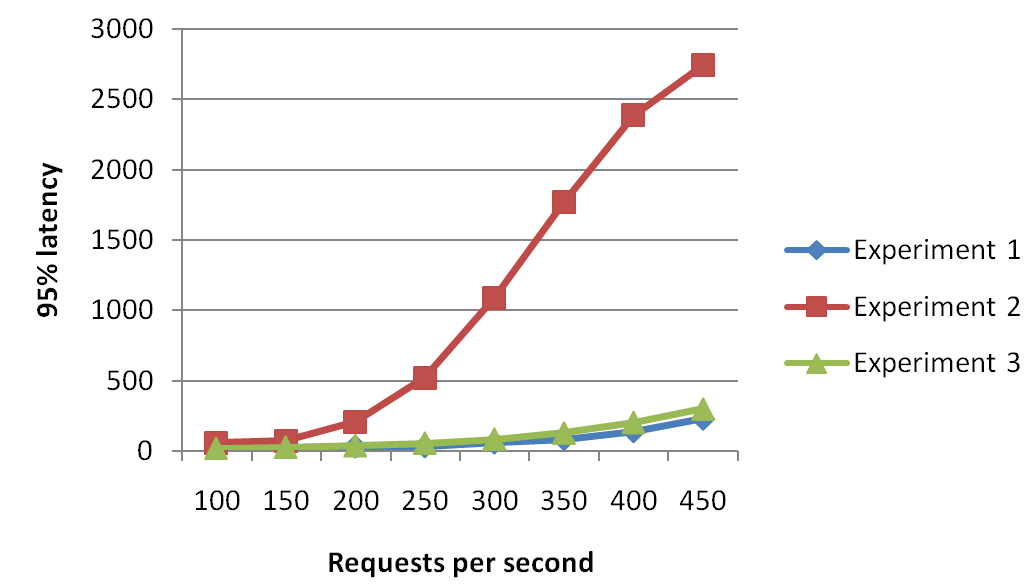
\includegraphics[width=0.90\columnwidth]{Images/Experiments/CPU/Latencies/lat-exp1-3.PNG}
\caption{95th percentile latencies during Experiment 1. At around 400 requests per second, the proposed SLO is violated.}
\label{fig:lat-cas-li} 
\end{figure}

\begin{figure}
\centering
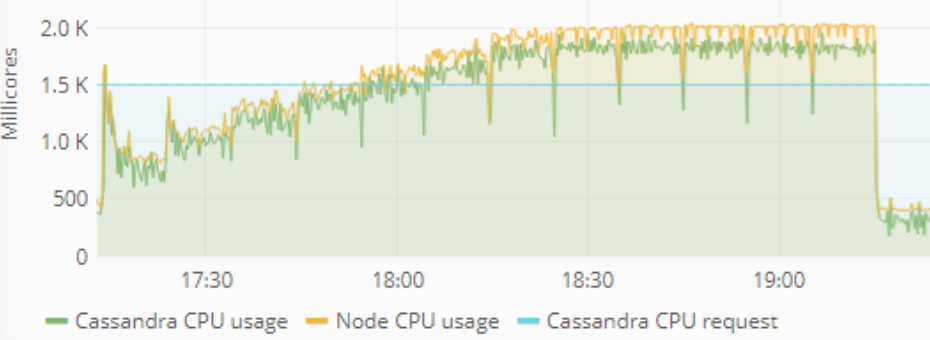
\includegraphics[width=0.80\columnwidth]{Images/Experiments/CPU/Grafana/cpu-cas-li.PNG}
\caption{Worker node CPU usage during Experiment 1. The CPU usage of Cassandra rises above its CPU request, illustrating that the application is able to use all of the overprovisioned resources.}
\label{fig:cpu-cas-li} 
\end{figure}

%It should be verified that the experiment controller has sufficient resources to run the experiments. Preliminary tests show that the experiment-controller is CPU bound. Figure \ref{fig:cpu-scalar} shows the experiment controller's CPU usage during the experiment described above. A peak in CPU usage can be examined at the start of each run, but these peaks stay well below the available amount of CPU in the node. The experiment controller should thus not be the bottleneck during the experiments.
%
%\begin{figure}
%\centering
%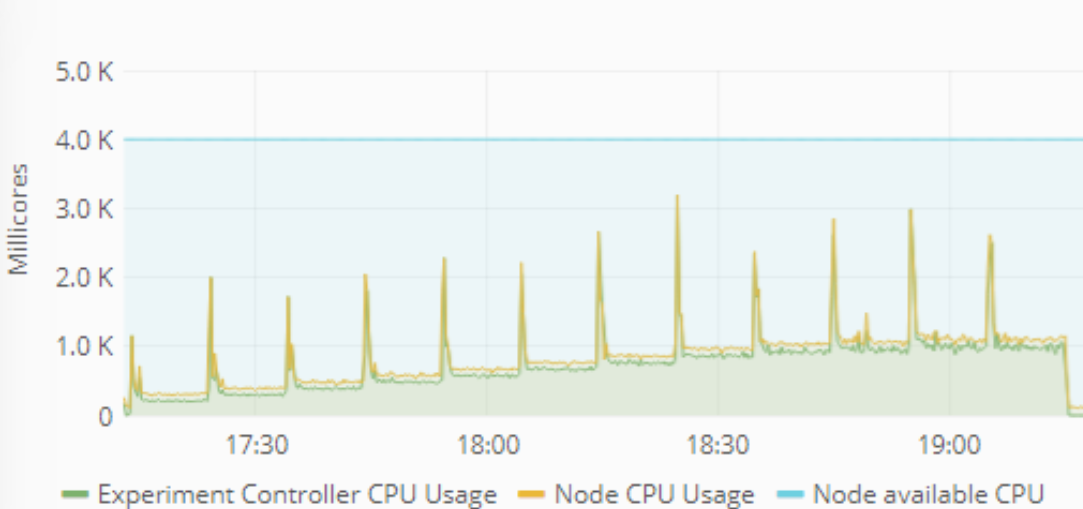
\includegraphics[width=0.80\columnwidth]{Images/Experiments/CPU/Grafana/cpu-scalar.PNG}
%\caption{Experiment controller CPU usage during Experiment 1. The node's CPU usage never reaches its capacity.}
%\label{fig:cpu-scalar} 
%\end{figure}

\subsection{Experiment 2: Determining the effects of co-locating a high and low priority application}
The goal of this experiment is to answer whether it is possible to increase cost-efficiency by using the Kubernetes oversubscription mechanisms described in Section 1. Through two tests, we illustrate the effects of different request configurations when a high and low priority pod are co-located on a node.

\subsubsection{Setup}
Compared to the first experiment, the application described in Section \ref{setup:lpp} is added to the second worker node as a low priority pod. The experiment consists of two separate tests. During the first one, the Cassandra application and the low priority pod each have a CPU request of \textit{500m}. For the second test, Cassandra has a CPU request of \textit{1500m} while the low priority pod has a CPU request of only \textit{10m}. The workload applied is the same as the one applied during Experiment 1. During the first test, both pods should receive an equal amount of CPU cycles. The results of the the test should indicate significantly higher 95th percentile latencies when compared to the results from Experiment 1, because the Cassandra pod cannot use all of the resources on the node. During the second test, Cassandra's performance should only be affected slightly as a result of the aforementioned \textit{cpu-shares} mechanism.

\subsubsection{Results}
Figure \ref{fig:cpu-cas-lpp-li} shows the CPU usage of both the Cassandra pod and the low priority pod during the first test, when their requests are equal. It shows that the available CPU is split equally between both pods. As expected, Figure \ref{fig:lat-cas-li} illustrates that the SLO posed earlier gets violated at about half the amount of requests per second when compared to Experiment 1.

\begin{figure}
\centering
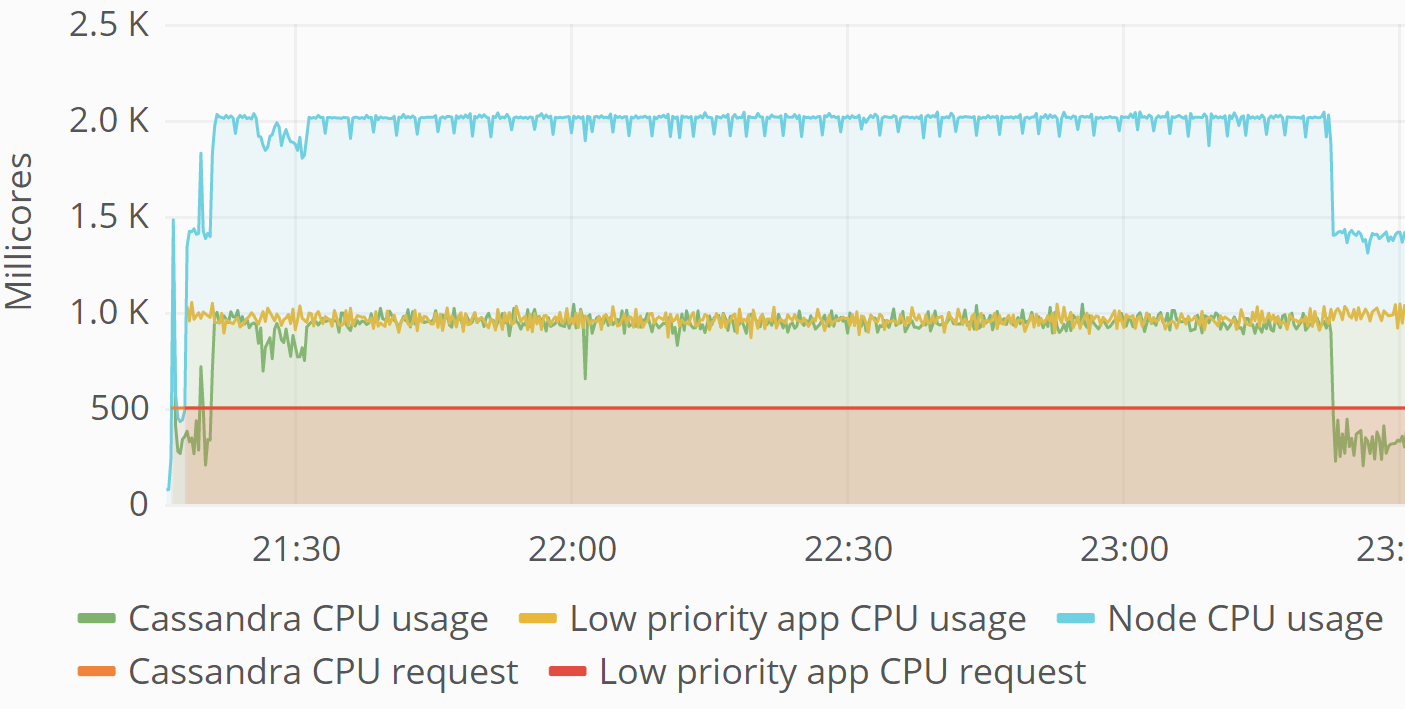
\includegraphics[width=0.90\columnwidth]{Images/Experiments/CPU/Grafana/cpu-cas-lpp-li.PNG}
\caption{Worker node CPU usage during the first test of Experiment 2. The deployed applications have an equal CPU request, resulting in them receiving an equal share of the available CPU.}
\label{fig:cpu-cas-lpp-li}
\end{figure}

%\begin{figure}
%\centering
%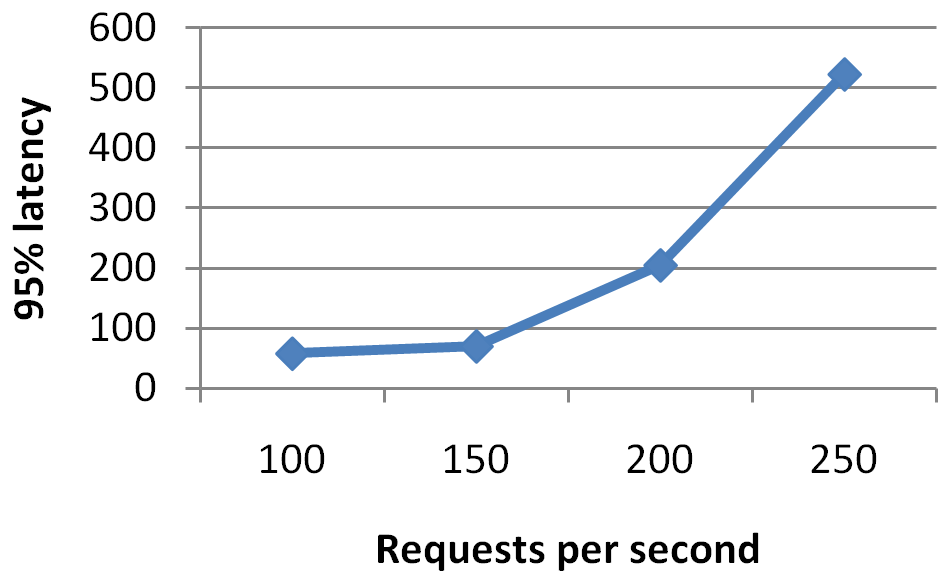
\includegraphics[width=0.50\columnwidth]{Images/Experiments/CPU/Latencies/lat-cas-lpp-li.PNG}
%\caption{95th percentile latencies during the first test of Experiment 2. The proposed SLO is violated at around 200 requests per second. Compared to Experiment 1, %the Cassandra application is able to process only half the amount of requests per second as a result of it only having access to half of the resources.}%
%\label{fig:lat-cas-lpp-li}
%\end{figure}
%
During the second test, the Cassandra pod should receive the vast majority of the available CPU when it needs to process a high workload. Figure \ref{fig:cpu-cas-lpp-li-2} shows the worker node's CPU usage during this test. As the amount of CPU needed by the Cassandra pod increases, the amount of CPU available to the low priority pod decreases, which is according to expectations. The 95th percentile latencies are shown in Figure \ref{fig:lat-cas-li}. The proposed SLO is breached between 350 and 400 requests per second. This is slightly lower when compared to the Experiment 1, where SLO violations started occurring at about 400 requests per second.

%\begin{figure}
%\centering
%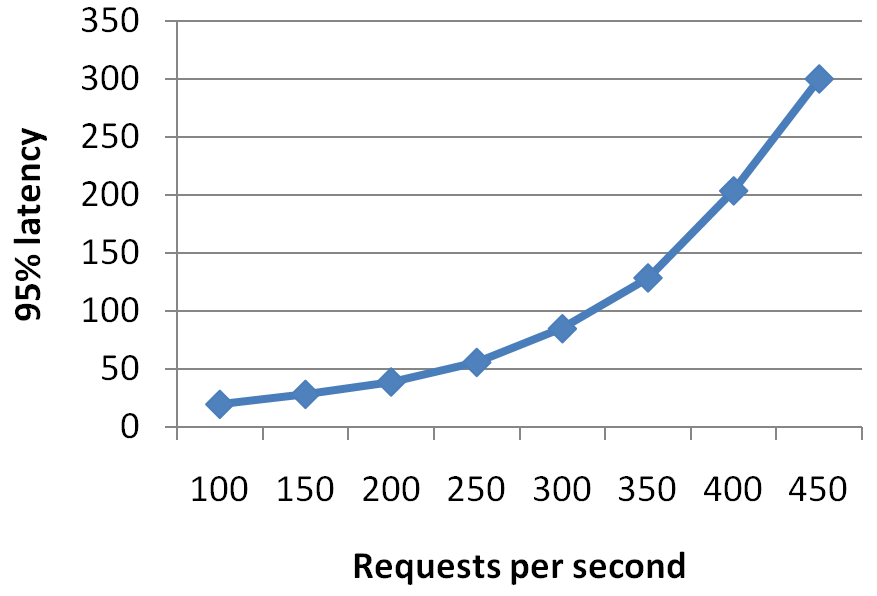
\includegraphics[width=0.50\columnwidth]{Images/Experiments/CPU/Latencies/lat-cas-lpp-li-2.PNG}
%\caption{95th percentile latencies during the second test of Experiment 2. The latencies are comparable to the ones examined during Experiment 1, showing that %performance is only slightly impacted.}
%\label{fig:lat-cas-lpp-li-2}
%\end{figure}

The slight decrease in performance comes with the benefit of a higher resource utilization. Comparing the worker node's total CPU usage during Experiment 1 to the node's total CPU usage during this test, in Figure \ref{fig:cpu-cas-lpp-li-2}, the latter shows a significantly higher resource utilization when the workload of the Cassandra pod is low.

\begin{figure}
\centering
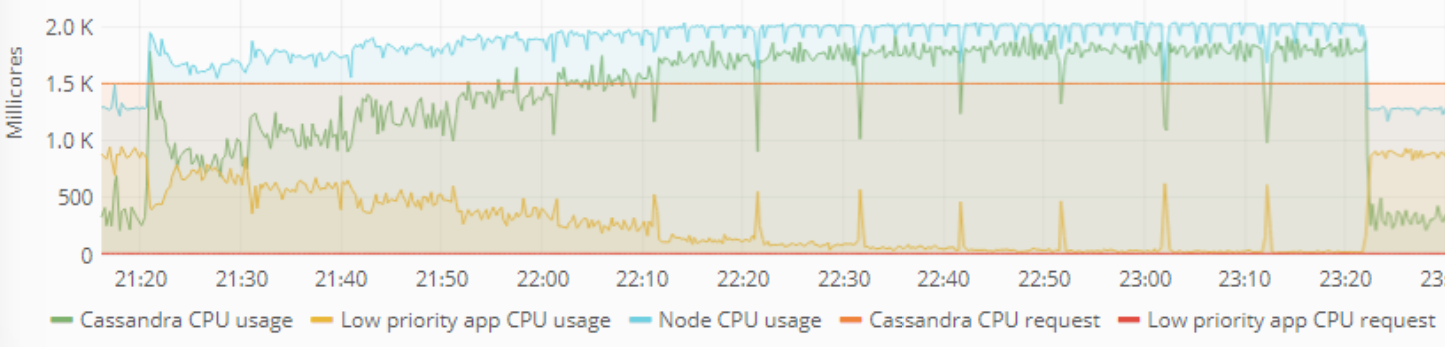
\includegraphics[width=\columnwidth]{Images/Experiments/CPU/Grafana/cpu-cas-lpp-li-2.PNG}
\caption{Worker node CPU usage during the second test of Experiment 2. As the Cassandra workload rises, the amount of CPU cycles granted to the low priority application decreases and vice versa. This increases cost-efficiency without heavily impacting the amount of CPU available to the Cassandra application.}
\label{fig:cpu-cas-lpp-li-2}
\end{figure}

\subsection{Experiment 3: Determining the effects of bursty workloads}
In this experiment, a bursty workload is applied to examine its effects on Cassandra's performance. In the previous experiment, Cassandra was able to process 350 requests per second without violating the proposed SLO. This experiment should clarify whether Kubernetes is able to divide resources in time so that Cassandra is able process the bursts of 350 requests per second without violating the SLO.

\subsubsection{Setup}
The setup for this experiment is equal to the one used in Experiment 2. In this experiment, K8-Scalar applies 5 minutes of a manageable workload (200 requests per second) followed by a one minute burst of 350 requests per second. This pattern is repeated 20 times.  

\subsubsection{Results}
Figure \ref{fig:cpu-cas-lpp-bursty} shows the node's resource utilization during this experiment. It depicts the expected behavior: during bursts in the workload, Cassandra's CPU usage increases rapidly, while the low priority pod's CPU usage changes inversely. The experiment controller reported an average 95th percentile latency of \textit{109.3 ms} during the bursts, which is comparable to the latencies reported during the previous experiment at 350 requests per second. The type of workload, bursty or more seasonal, thus seems to have no effect on the operation of the \textit{cpu-shares} mechanism. Futhermore, adding a low priority pod increases cost-efficiency in between bursts.

\begin{figure}
\centering
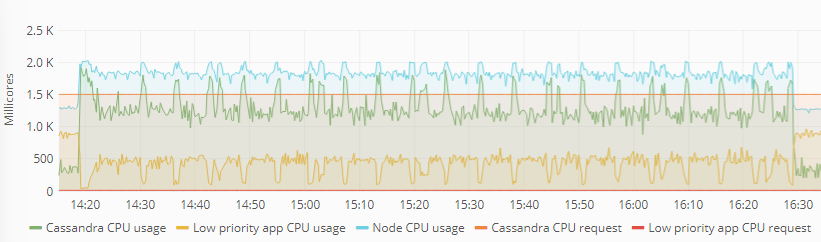
\includegraphics[width=\columnwidth]{Images/Experiments/CPU/Grafana/cpu-cas-lpp-bursty.PNG}
\caption{Worker node CPU usage during Experiment 3. During a burst, CPU cycles are taken away from the low priority application and granted to the high priority one. The low priority application is allowed to use more resources in between bursts, increasing cost-efficiency.}
\label{fig:cpu-cas-lpp-bursty}
\end{figure}

\subsection{Experiment 4: Determining the effects of the Kubernetes HPA on Cassandra performance}
\label{exp:hpa-cass}
When the resources available to an applications are insufficient for it to meet its QoS requirements, replicas may need to be added. An application should be able to handle significantly more workload if it is able to scale out. The goal of this experiment is to validate the correct performance of the HPA in combination with the application at hand, Cassandra. 

\subsubsection{Setup}
In this experiment, the HPA is added to the cluster, and the third worker node is made available to deploy a replica of the Cassandra application on. The low priority pod is removed from the cluster. The workload described in Experiment 1 will be applied to Cassandra. The HPA is configured to scale Cassandra when its CPU usage rises above 110\% of its CPU request, so at around \textit{1650 millicores}. 110\% is selected as the point to scale as spinning up a new replica takes some time. Scaling when the node's resources are fully used may be too late and may thus result in SLA violations. The experiment controller divides the workload among all active replicas by sending the requests to the Cassandra application service, which takes care of the load balancing. 

\subsubsection{Results}
Figure \ref{fig:cpu-cas-hpa-li} shows the CPU usage of the primary Cassandra pod and the replica added by the HPA. The graphs indeed illustrate that a new Cassandra replica is added when the original one uses approximately \textit{1650 millicores}. Despite this, the load on the original Cassandra replica does not decrease when the new replica is activated. Since the experiment controller sends the workload to the Cassandra service, and this service should load balance over all available replicas, this is not in line with expectations. The CPU usage of the original replica should decrease when a new replica is available. The 95th percentile latencies of the requests, depicted in Figure \ref{fig:lat-cas-hpa-li}, reflect this unexpected behavior. Instead of the latencies going down when a new replica is added, they go up significantly. This can partially be explained by the fact that there is a certain warm-up associated with new Cassandra replicas: the first requests sent to a new Cassandra replica have higher latencies. This short-lived warm-up period explains the peak in latencies around 400 requests per second (the point of scaling), but does not justify the whole picture. The full explanation is beyond the scope of this paper but in short, Truyen et al.~\citep{TruyenEddy2019Pooc} found that Kubernetes introduces a performance overhead when running Cassandra. %Additional experiments performed during this paper illustrated that this performance overhead increases significantly when more replicas are added. Scaling Cassandra in a native deployment, without using Kubernetes, did not cause major performance losses. In conclusion, the overhead was shown not to be caused by the HPA algorithm, but by Kubernetes itself.

\begin{figure}
\centering
\begin{subfigure}[b]{\columnwidth}
\centering
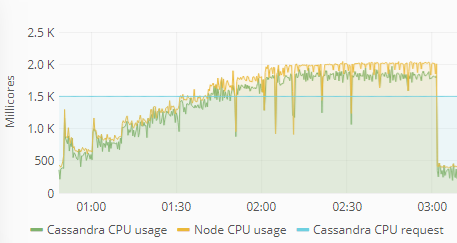
\includegraphics[width=0.70\columnwidth]{Images/Experiments/CPU/Grafana/cpu-cas-hpa-li-1.PNG}
\caption{First worker node's CPU usage}
\label{fig:cpu-cas-hpa-li-1}
\end{subfigure}
\hfill
\begin{subfigure}[b]{\columnwidth}
\centering
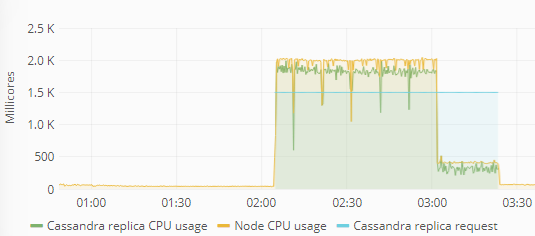
\includegraphics[width=0.70\columnwidth]{Images/Experiments/CPU/Grafana/cpu-cas-hpa-li-2.PNG}
\caption{Second worker node CPU usage}
\label{fig:cpu-cas-hpa-li-2}
\end{subfigure}
\hfill
\caption{CPU usage during Experiment 4. At 110\% of the CPU request, the given CPU threshold, a new Cassandra replica is added by the HPA. The CPU usage of the original replica does not decrease when the new replica is added, indicating scalability issues of Cassandra in Kubernetes.}
\label{fig:cpu-cas-hpa-li}
\end{figure}

\begin{figure}
\centering
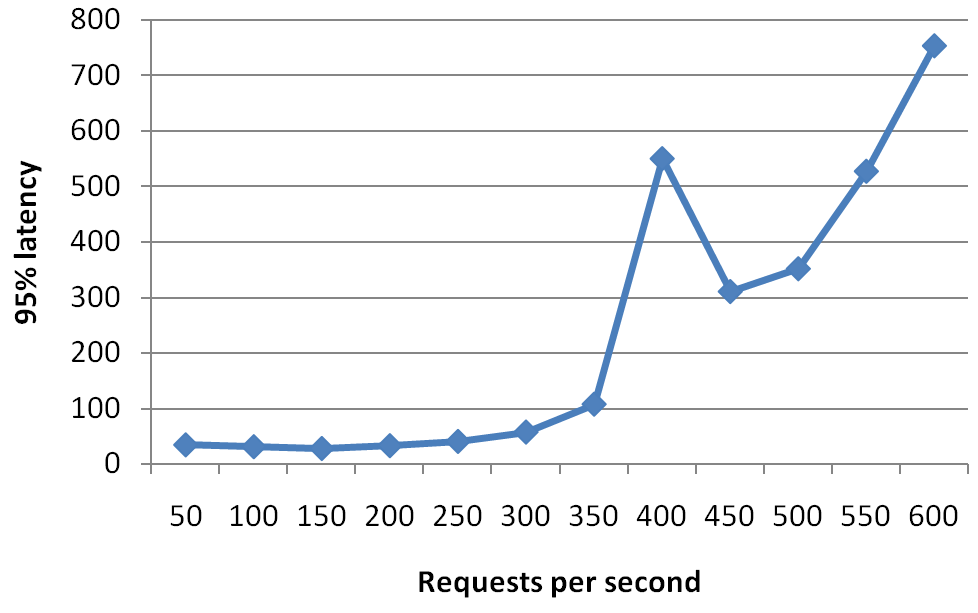
\includegraphics[width=0.55\columnwidth]{Images/Experiments/CPU/Latencies/lat-cas-hpa-li.PNG}
\caption{95th percentile latencies during Experiment 4. The latencies increase rather than decrease when a replica is added, confirming the scalability issues of Cassandra in Kubernetes.}
\label{fig:lat-cas-hpa-li}
\end{figure}

\subsection{Experiment 5: Determining the effects of the Kubernetes HPA on the SaaS application performance}
The previous experiment is redone with the artificial SaaS application (introduced in Section \ref{setup:saas-app}) replacing Cassandra. Through two tests, this experiment verifies whether the performance of the SaaS application increases after a replica is added, or if it encounters the same scalability issues in Kubernetes as Cassandra.  

\subsubsection{Setup}
The SLO posed for the SaaS application is equal to the one posed for the Cassandra application in Experiment 1. Two separate tests are run. The first one subjects the SaaS application to a linearly increasing workload to see how much requests one replica can handle. The SaaS application's CPU request is set to 1.5 CPU. The linearly increasing workload applied to the SaaS application starts at 50 requests per second and increases with 50 requests per second each 600 seconds, up to 300 requests per second. For the second test, the HPA is added to the cluster and linearly increasing workload is again applied to the SaaS application. The workload now rises up to 600 requests per second instead of up to 300. Again, 110\% is selected as the point of scaling for the HPA. 


\subsubsection{Results}
Figure \ref{fig:lat-saas-li} shows the 95th percentile of latencies during the first test. The SaaS application is able to process 150 requests per second without violating the SLO. Figure \ref{fig:cpu-saas-li} illustrates that at around 150 requests per second, the CPU in the node is fully used up, confirming that CPU is the bottleneck. 

\begin{figure}
\centering
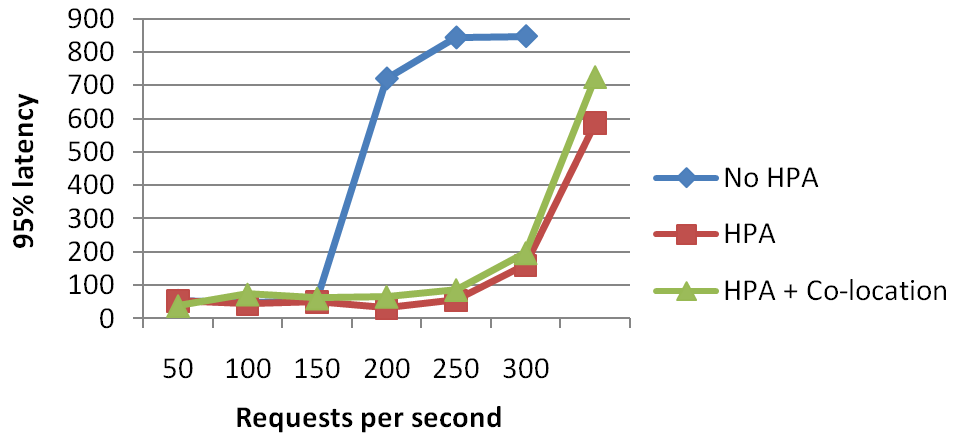
\includegraphics[width=0.95\columnwidth]{Images/Experiments/CPU/Latencies/lat-exp5-7.PNG}
\caption{95th percentile latencies during the first test of Experiment 5. The application is able to process 150 requests per second without violating the SLO, but not 200 requests per second.}
\label{fig:lat-saas-li}
\end{figure}

\begin{figure}
\centering
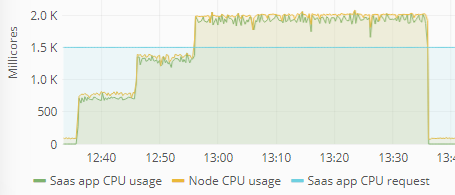
\includegraphics[width=0.75\columnwidth]{Images/Experiments/CPU/Grafana/cpu-saas-li.PNG}
\caption{Worker node CPU usage during the first test of Experiment 5. The resources of the node are fully used up at 150 requests per second. Since the SaaS application cannot acquire the resources needed to process 200 requests per second, the SLO gets violated.}
\label{fig:cpu-saas-li}
\end{figure}

Figure \ref{fig:lat-saas-li} shows the latencies during the second test of this experiment. These illustrate that the SaaS application is able to process 250 requests per second without violating the SLO. This slightly less than double the 150 requests per second which the SaaS application can process without the HPA. Hence, there is still some overhead associated with having multiple replicas of the SaaS application, but it is relatively small compared to the overhead detected when scaling Cassandra in Kubernetes. Figure \ref{fig:cpu-cas-hpa-li-2} confirms that the workload is distributed over the replicas.
%
%\begin{figure}
%\centering
%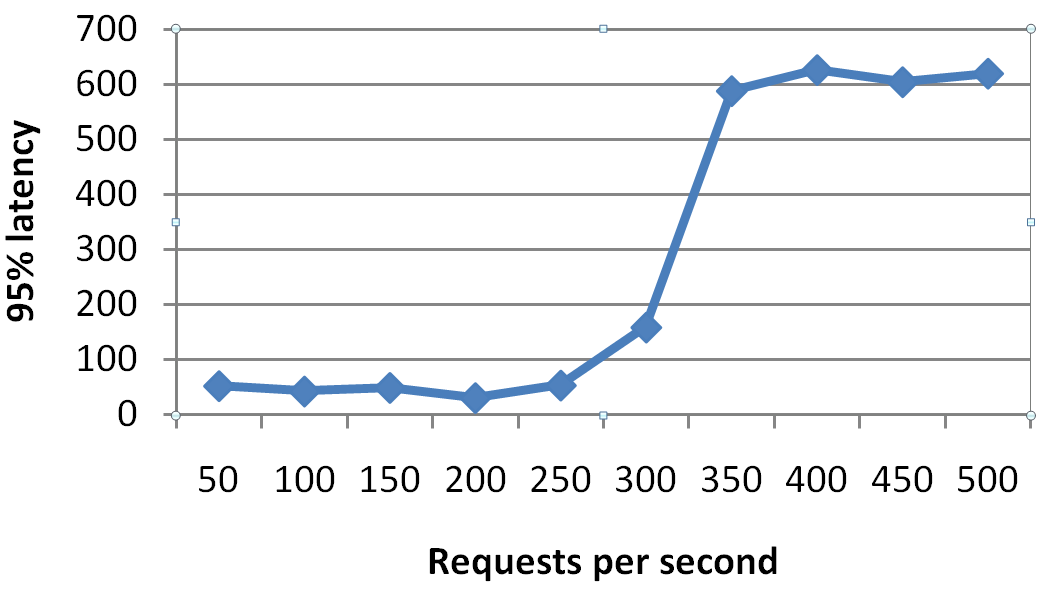
\includegraphics[width=0.60\columnwidth]{Images/Experiments/CPU/Latencies/lat-saas-hpa-li.PNG}
%\caption{95th percentile latencies during the second test of Experiment 5. The SaaS application can process a significantly higher amount of requests per second if an extra replica is added.}
%\label{fig:lat-saas-hpa-li}
%\end{figure}


\begin{figure}
\centering
\begin{subfigure}[b]{\columnwidth}
\centering
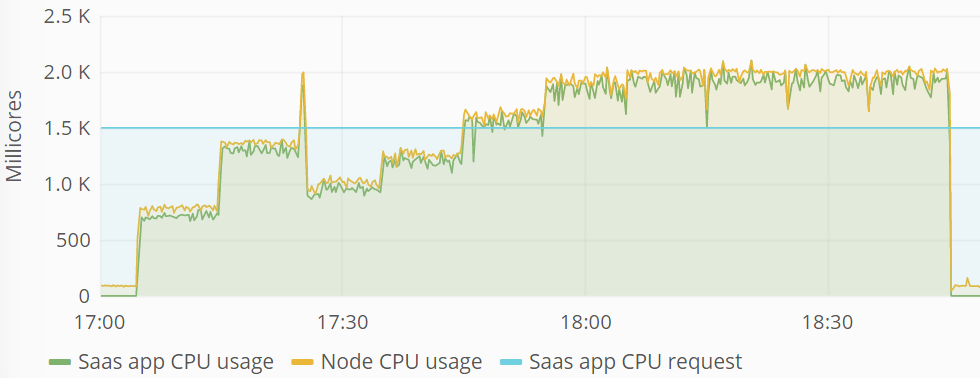
\includegraphics[width=0.75\columnwidth]{Images/Experiments/CPU/Grafana/cpu-saas-hpa-li-1.PNG}
\caption{First worker node's CPU usage during the second test of Experiment 5.}
\label{fig:cpu-saas-hpa-li-1}
\end{subfigure}
\hfill
\begin{subfigure}[b]{\columnwidth}
\centering
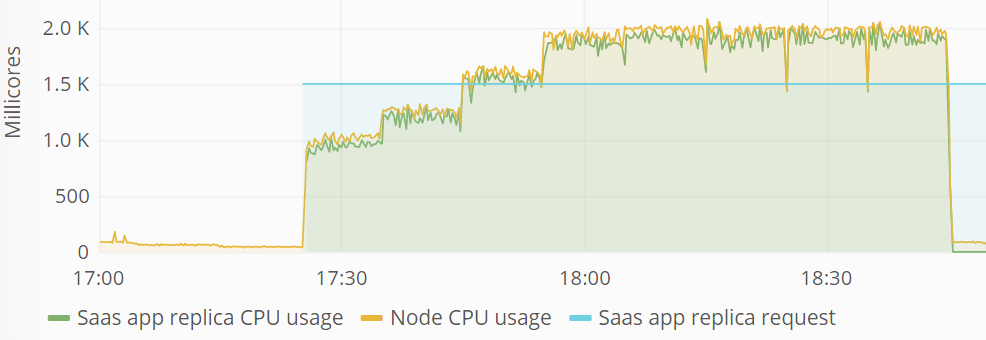
\includegraphics[width=0.75\columnwidth]{Images/Experiments/CPU/Grafana/cpu-saas-hpa-li-2.PNG}
\caption{Second worker node's CPU usage}
\label{fig:cpu-saas-hpa-li-2}
\end{subfigure}
\hfill
\caption{CPU usage during the second test of Experiment 5. The CPU usage of the original replica decreases when the HPA schedules a new replica of the SaaS application, confirming that the load is distributed among all replicas.}
\label{fig:cpu-cas-hpa-li-2}
\end{figure}

\subsection{Experiment 6: Determining the effects of bursty workloads on the performance of the Kubernetes HPA}
The goal of this experiment is to test how the Kubernetes HPA performs when the workload is bursty rather than linearly increasing. Even with the HPA added to the cluster, the SaaS application might not be able to process bursts of 250 requests per second, since starting a new replica can be slow. The burst could be over by the time that the replica is fully started up.

\subsubsection{Setup}
The setup for this experiment is the same as the one used during the second test of the previous experiment. The bursty workload applied consists of five minutes of 60 requests per second followed by a one minute peak of 250 requests per second. This pattern is repeated 20 times.  

\subsubsection{Results}
Figure \ref{fig:cpu-saas-hpa-bursty} show the worker node's CPU usages during this experiment. The graphs illustrate that during the first couple of bursts, no scaling happens. This is unexpected. The 95th percentile latencies also report SLA violations during these bursts. One possible explanation is that the HPA does not poll the resource usage during the burst and thus does not notice the burst. This is, however, not the case, since the HPA queries the resource utilization every 15 seconds by default, and a burst lasts for 60 seconds. The HPA's algorithm details~\citep{hpa-algorithm-details} proved insufficient to find the cause of this behavior.


\begin{figure}
\centering
\begin{subfigure}[b]{\columnwidth}
\centering
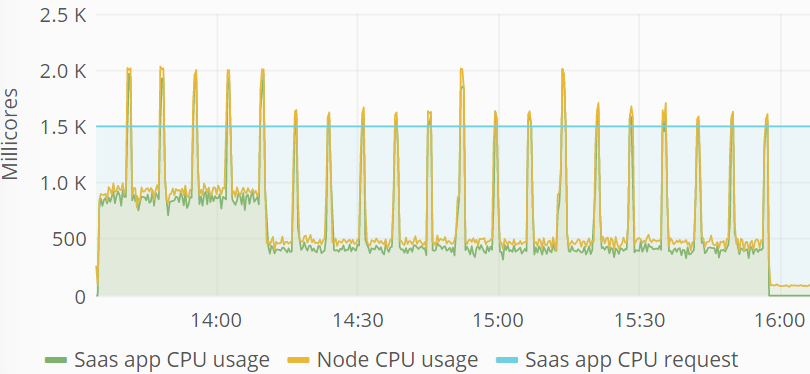
\includegraphics[width=0.75\columnwidth]{Images/Experiments/CPU/Grafana/cpu-saas-hpa-bursty-2-1.PNG}
\caption{First worker node's CPU usage.}
\label{fig:cpu-saas-hpa-bursty-2-1}
\end{subfigure}
\hfill
\begin{subfigure}[b]{\columnwidth}
\centering
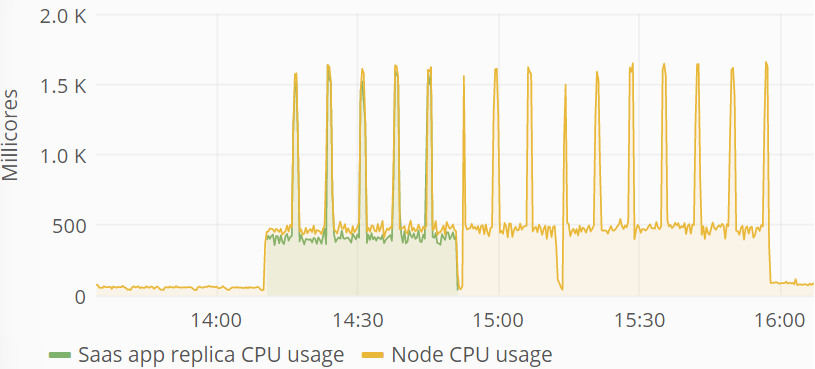
\includegraphics[width=0.75\columnwidth]{Images/Experiments/CPU/Grafana/cpu-saas-hpa-bursty-2-2.PNG}
\caption{First worker node's CPU usage.}
\label{fig:cpu-saas-hpa-bursty-2-2}
\end{subfigure}
\hfill
\caption{CPU usage during the first test of Experiment 6. The HPA does not schedule a new replica of the SaaS application until the 5th burst. After that, the replica is removed and rescheduled multiple times. When a new replica is scheduled or removed, is seemingly random. }
\label{fig:cpu-saas-hpa-bursty}
\end{figure}

Another observation made from this experiment's results is that the HPA does not scale the application down after each burst. The HPA calculates the desired amount of replicas as follows~\citep{hpa-algorithm-details}:

\[ desiredReplicas = ceil[currentReplicas\ *\ (\ currentValue\ /\ desiredValue\ )] \]

The \textit{desiredValue} was set to \textit{110\%} of the request, so approximately \textit{1650m}. The \textit{currentValue} is calculated by ``taking the average of the given metric across all pods in the HorizontalPodAutoscaler's scale target''~\citep{hpa-algorithm-details}. In between bursts, figures \ref{fig:cpu-saas-hpa-bursty-2-1} and \ref{fig:cpu-saas-hpa-bursty-2-2} show that this value is around \textit{500m}. Given these values, the number of desired replicas is one.

It is possible that the HPA does not scale down the SaaS application due to the default \textit{downscale stabilization} parameter of the HPA algorithm being five minutes~\citep{hpa-cooldown-delay}. This parameter specifies a period of time during which the HPA considers all recommendations before scaling down. In other words, the HPA only scales down if its decision to scale down has not changed for five minutes. The downtime during each burst in this experiment was set to exactly five minutes. Since the HPA should not scale down during a burst, this could lead to the HPA not scaling down at all. Combined with the knowledge that the metrics get queried only every 15 seconds, this could also explain why the HPA did scale down during the 11th and 14th burst.

To verify these assumptions, another test is run in which the downtime between each burst is set to 7 minutes. The other experiment parameters remain unchanged. Figure \ref{fig:cpu-saas-hpa-bursty-2} show the CPU usage of the two worker nodes. During this test, the HPA scaled up the SaaS application during the first burst, but did not scale it down until after the test was completed. 

\begin{figure}
\centering
\begin{subfigure}[b]{\columnwidth}
\centering
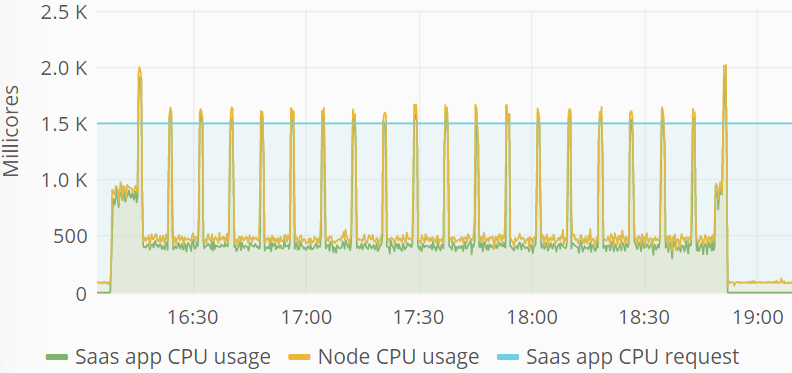
\includegraphics[width=0.70\columnwidth]{Images/Experiments/CPU/Grafana/cpu-saas-hpa-bursty-3-1.PNG}
\caption{First worker node's CPU usage.}
\label{fig:cpu-saas-hpa-bursty-3-1}
\end{subfigure}
\hfill
\begin{subfigure}[b]{\columnwidth}
\centering
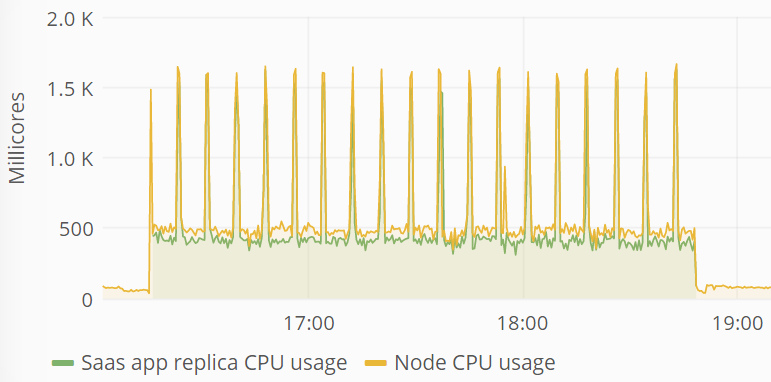
\includegraphics[width=0.70\columnwidth]{Images/Experiments/CPU/Grafana/cpu-saas-hpa-bursty-3-2.PNG}
\caption{First worker node's CPU usage.}
\label{fig:cpu-saas-hpa-bursty-3-2}
\end{subfigure}
\hfill
\caption{CPU usage during the second test of Experiment 6. Increasing the time between bursts results in the HPA scaling a new replica during the first burst. This replica is not removed until the test is over.}
\label{fig:cpu-saas-hpa-bursty-2}
\end{figure}

Neither these experimental results nor the official documentation about the HPA~\citep{hpa-algorithm-details} clarify how the HPA decides when to scale an algorithm. Discovering the cause of this unexpected behavior is left for future work. The results show, however, that the HPA is unfit to process bursty workloads effectively.


\subsection{Experiment 7: Determining the effects of combining the Kubernetes HPA with the presence of a low priority pod}
Experiment 2 illustrated that co-locating a high and low priority pod has a minor impact on the high priority application's performance, while in increases the overall cost-efficiency. The goal of this experiment is to test whether this is still the case when the HPA is added to the cluster. 

\subsubsection{Setup}
The scaling point for the SaaS application is again set to 110\%. The application is subjected to the linearly increasing workload described in Experiment 5.


\subsubsection{Results}
Figure \ref{fig:lat-saas-li} shows the 95th percentile latencies recorded during this experiment. They are only slightly higher compared to the latencies recorded during Experiment 5. This slight decrease in performance again comes with the benefit of a higher resource utilization during low workloads, as illustrated by Figure \ref{fig:cpu-saas-lpp-hpa-li-1}. The low priority pod is able to use the excess of resources on the node during low workloads. As the workload rises, the low priority pod is given access to less CPU cycles. When a new replica of the SaaS application is added to the cluster, the amount of requests which the original replica needs to process lowers, again freeing up resources for the lower priority pod to use. 

%\begin{figure}
%\centering
%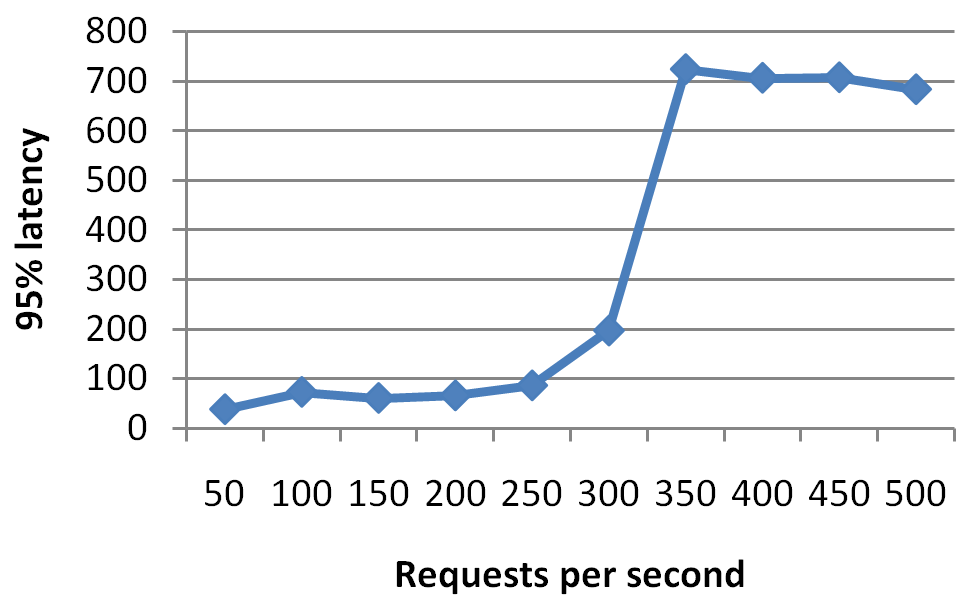
\includegraphics[width=0.60\columnwidth]{Images/Experiments/CPU/Latencies/lat-saas-lpp-hpa-li.PNG}
%\caption{95th percentile of latencies during experiment 7. They are only slightly higher than the ones recorded during Experiment 5. This indicates that adding a %co-locating a high and low priority pod increases cost-efficiency, even when the high priority pod is able to scale.}
%\label{fig:lat-saas-lpp-hpa-li}
%\end{figure}
%
%
\begin{figure}
\centering
\begin{subfigure}[b]{0.9\columnwidth}
\centering
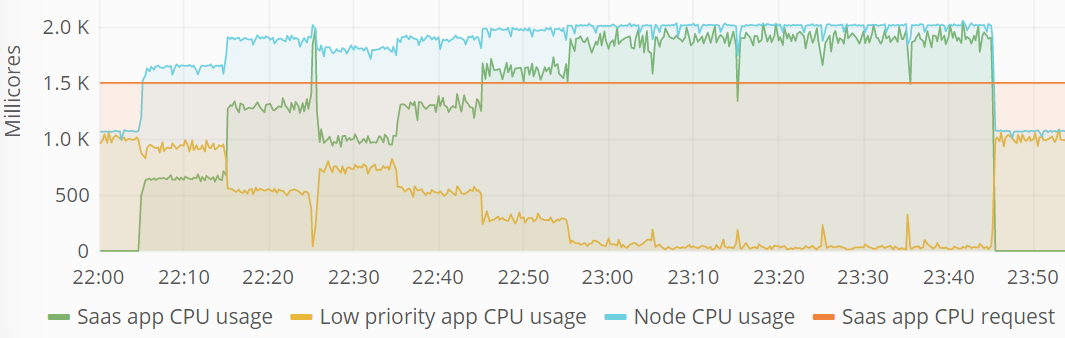
\includegraphics[width=0.75\columnwidth]{Images/Experiments/CPU/Grafana/cpu-saas-lpp-hpa-li-1.PNG}
\caption{First worker node's CPU usage.}
\label{fig:cpu-saas-lpp-hpa-li-1}
\end{subfigure}
\hfill
\begin{subfigure}[b]{0.9\columnwidth}
\centering
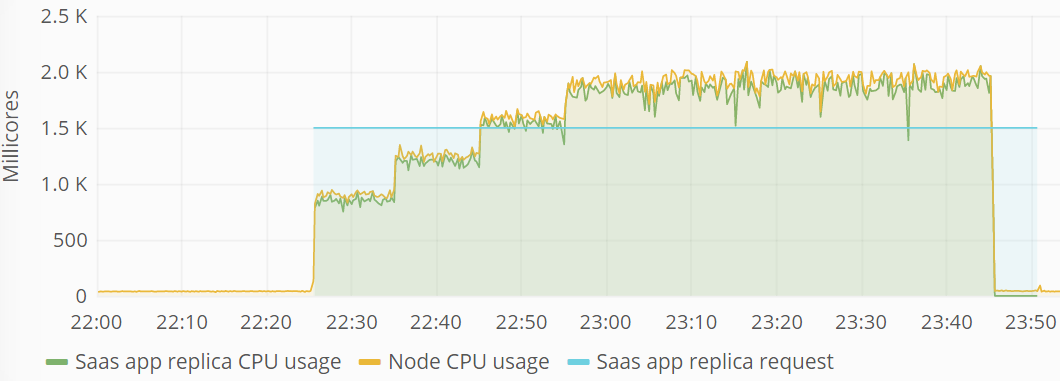
\includegraphics[width=0.75\columnwidth]{Images/Experiments/CPU/Grafana/cpu-saas-lpp-hpa-li-2.PNG}
\caption{First worker node's CPU usage.}
\label{fig:cpu-saas-lpp-hpa-li-2}
\end{subfigure}
\hfill
\caption{CPU usage during Experiment 7. The resource utilization of the node increases by adding a low priority pod without heavily impacting the amount of resources to which the high priority pod has access.}
\label{fig:cpu-saas-lpp-hpa-li}
\end{figure}
